\section{Methodology}\label{sec:chap4 methodology}

\subsection{Data generation}
We study ensembles of redistricting plans $x$ distributed according to a measure of interest:
    \begin{align}
        \pi(x)\propto e^{-J(x)},
    \end{align}
where $J$ is a score function that reflects the hard and soft constraints for a desirable redistricting plan, e.g., population deviation, connectedness, etc.
To efficiently obtain plan samples from $\pi$, we use the Metropolized Cycle Walk~\cite{cyclewalk}.
Each step modifies a spanning forest (on $G$) by adding an edge $e$ and removing a random edge on the cycle created by $e$.
We then accept or reject the resulting forest using a standard Metropolis-Hastings acceptance rule that satisfies detailed balance.
After burn-in, we collect $M$ observations $\mathcal{X}_{obs}:=\{x^{(m)}\}_{m=1}^M$ from the chain output every $100$ steps.

Recall that each plan $x^{(m)}$ is an unordered tuple of $I$ districts in $\mathcal{V}$. 
Pooling districts across the $M$ plans yields a set of $N$ districts
\begin{align}
    \mathcal{D} := \{v_1,\dots,v_N\}\subset \mathcal{V},
\end{align}
where $N\leq MI$ because plans may contain exactly same districts.
We compute the pairwise district-to-district distances according to \eqref{eq:dist_district} and store them in coordinate (COO) format, which is convenient for the clustering algorithms that we use.
This approach saves memory because we only store the distances below $d_{max}$, especially when $I$ is large.

\subsection{Building letters}
To find representative districts (``letters''), we cluster the pooled district set $\mathcal{D}$ with \hccultra~\cite{DBLP:journals/corr/abs-2409-01010}, which is a hierarchical correlation clustering algorithm that comes with nice theoretical guarantees.
To scale the algorithm to large graphs, we optimize memory usage by tracking only the active roots during merging, which avoids storing a dense $2N\times 2N$ matrix as in a naive implementation.
The most time-consuming step is sorting the edges by distance.
We therefore bucket-sort the COO distances and parallelize across bins, where bin boundaries are estimated from a small pilot sample.
This produces a single dendrogram, which we can cut to obtain clustering for any desired $K$.

To choose $K$, we use the elbow method on a dispersion objective $\mathcal{L}(K)$.
Let $\mathcal{D}_1,\mathcal{D}_2,\dots,\mathcal{D}_K$ be the clusters, i.e., a partition of $\mathcal{D}$.
For each cluster, we define its letter (centroid) $l_k\in\{0,1\}^P$ as the point that minimizes the sum of distances to members of $\mathcal{D}_k$:
\begin{align}\label{eq:centroid definition}
    l_k &:= \arg\min_{l\in\{0,1\}^P}\sum_{v\in\mathcal{D}_k}d(l,v),\\
\end{align}
Under weighted $l^1$ distance \eqref{eq:dist_district}, this reduces to a precinct-wise median:
\begin{align}
    (l_k)_p &=
    \begin{cases}
        1, & \sum_{v\in\mathcal{D}_k} v_p \ge \frac{|\mathcal{D}_k|}{2},\\
        0, & \text{otherwise,}
    \end{cases}
    \qquad p=1,\dots,P.
\end{align}
Given the letters $l_1,\dots,l_K$, we score the clustering via the within-cluster dispersion
\begin{align}\label{eq:dispersion_obj}
    \mathcal{L}(K) &:= \sum_{k=1}^K \sum_{v\in\mathcal{D}_k} d(v,l_k),
\end{align}
an $\ell^1$ analogue of within-cluster sum of squares (WCSS), which is a common metric for choosing the number of clusters.
Empirically, we find that $\mathcal{L}(K)$ is strongly correlated with standard alternatives such as the Silhouette score, the Calinski--Harabasz index, and BCSS, as well as information-theoretic objectives like BIC and AIC.

\subsection{From letters to words}\label{subsec:letters_to_words}
After clustering districts into an alphabet $\{l_1,\dots,l_K\}$, we construct the set of words by taking the union of unordered $I$-tuples of letters around each plan $x\in\mathcal{X}$.
These candidate words serve two roles: they provide a compressed description of the plans, and they define the local support of the kernel $\psi$ in \eqref{eq:psi_relative} used for the partition of unity.
Observe that evaluating the plan-level distance \eqref{eq:dist_plan} between two arbitrary elements of $\mathcal{W}$ is computationally intractable, since it involves looping over all permutations of size $I$.
However, we can exactly enumerate $L$ closest neighbors for a point in $\mathcal{W}$ in $\mathcal{O}(IK\log L+K\log K)$ via beam search.

Let $v_1(x),\dots,v_I(x)$ be the districts of $x$.
For each district, we precompute a sorted list of letter candidates
\begin{align}\label{eq:district_to_letter_candidates}
    C_i(x) &:= \big(d_{v_i(x),l_k},l_k\big)_{k=1}^K,\qquad i=1,\dots,I,
\end{align}
where the pairs are sorted by increasing $d_{v_i(x),l_k}$.
During beam search, we incrementally build partial sub-words by adding one letter at a time, and keep only the $L$ best candidates at each step.
See Algorithm~\ref{alg:beam_search} for more details.
\begin{algorithm}[!htbp]
\caption{Beam search for nearest words with width $L$}
\label{alg:beam_search}
\begin{algorithmic}[1]
\Require For each district $i\in[I]$, a list $C_i=\{(d_{i,k}, \ell_{i,k})\}_{k=1}^K$ of candidate letters sorted by $d_{i,k}$
\State $B \gets [(0, [])]$ \Comment{beam of (distance, partial word)}
\For{$i=1$ \textbf{to} $I$}
    \State $H \gets$ empty max-heap keyed by negative distance \Comment{keeps track of $L$ minimum distances}
    \ForAll{$(D,s)\in B$}
        \ForAll{$(d,\ell)\in C_i$}
            \If{$\ell \in s$}
                \State \textbf{continue} \Comment{avoid repeated letters}
            \EndIf
            \State $D' \gets D + d$
            \State $s' \gets \mathrm{append}(s,\ell)$
            \State \Call{HeapPush}{$H,(D',s')$}
            \If{$\Call{HeapSize}{H} > L$}
                \State \Call{HeapPopMax}{H} \Comment{discard the current worst (largest-distance) candidate}
            \EndIf
        \EndFor
    \EndFor
    \State $B \gets$ elements of $H$ sorted by increasing distance
\EndFor
\State \Return $B$
\end{algorithmic}
\end{algorithm}

\begin{figure}[!htbp]
    \centering
    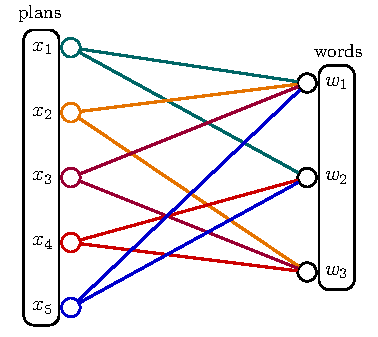
\includegraphics[width=0.55\linewidth]{figures/overlap/bipartite.pdf}
    \caption{Connectivity of a beam search with width $2$. Edges are colored by plans. Each observed plan on the left connects to the two closest words. In this example, we obtain three words in total.}
    \label{fig:overlap/bipartite}
\end{figure}
\FloatBarrier
For each observed plan $x$, we keep the $L$ best candidates as $w_1(x),\dots,w_L(x)$ and take the union of these sets across the ensemble to form the representitative word set $\mathcal{S}$ used for stratification.
It maybe helpful to treat plans and words as vertices and think of the beam search process as building the connections in a bipartite graph, as shown in Figure \ref{fig:overlap/bipartite}.

\subsection{Towards stratification}
The representative word set $\mathcal{S}$ and the plan-level distances $D$ allow us to construct a stratification of the target distribution $\pi$ on plans.
We start with a partition of unity (POU) $\{\phi_s\}_{s\in\mathcal{S}}$ and define the corresponding stratum distributions $\{\pi_s\}_{s\in\mathcal{S}}$ via tilting.
Each $\phi_s(x)$ can be interpreted as a soft-assignment of plan $x$ to stratum $s$, with flow between strata encoded by the flux matrix $F$ in \eqref{eq:flux}.

One key requirement for US to work is coverage, meaning that every plan should have at least one nearby word so that the POU is well-supported.
In our construction this is ensured by beam search, which yields $L$ candidate words $w_1(x),\dots,w_L(x)$ for each plan $x$ and restricts $\psi(x;s)$ in \eqref{eq:psi_relative} to this neighborhood.
Another important requirement of US is that strata have appropriate overlaps.
Some overlap is necessary for communication between strata, but excessively large overlap can lead to slow convergence (as well as numerical instability) of EMUS-style fixed-point iterations.
In practice, the temperature $T$ and the choice of $\kappa$ in \eqref{eq:psi_relative} are the primary control knobs that we can tune to reach desired coverage and overlap.
By construction, the induced coarse dynamics on $\mathcal{S}$ has stationary distribution $z$:
\begin{align}
    \pi(x) &= \sum_{s\in\mathcal{S}} z_s\,\pi_s(x),\qquad
    z^\top F = z^\top,
\end{align}
which we use as a diagnostic to see whether the strata design is fit for stratified sampling.

Actually running stratified sampling requires additional sampling work (e.g., parallel chains targeting $\{\pi_s\}$), whereas here we focus on setting up a reasonable stratification of plan space and the associated overlap statistics.
When overlap is very large and $\mathcal{S}$ becomes highly redundant, we may prune the strata by solving a set-cover problem induced by the plan--word bipartite graph.
Concretely, each word covers a subset of the observed plans, so the words define a family of subsets of the plan space.
The basic greedy subcover routine takes a boolean adjacency matrix $A\in\{0,1\}^{M\times|\mathcal{S}|}$ and repeatedly adds the word that covers the largest number of currently uncovered plans.
Selecting a minimum-size sub-collection $\mathcal{S}_0\subseteq\mathcal{S}$ can be written as
\begin{align}
    \min_{\mathcal{S}_0\subseteq\mathcal{S}} \quad & |\mathcal{S}_0|,\\
    \text{s.t.}\quad & \sum_{s\in\mathcal{S}_0} A_{m,s} \ge 1,\qquad m=1,\dots,M.
\end{align}
The problem of deciding whether there is a subcover smaller than some fixed size is NP-complete in general, so we use the greedy approximation in Algorithm~\ref{alg:greedy_subcover}.
\begin{algorithm}[!htbp]
\caption{Greedy subcover}
\label{alg:greedy_subcover}
\begin{algorithmic}[1]
\Require Adjacency matrix $A\in\{0,1\}^{M\times|\mathcal{S}|}$
\State $U \gets \{1,\dots,M\}$ \Comment{uncovered plan indices}
\State $R \gets \mathcal{S}$ \Comment{remaining candidate words}
\State $\mathcal{S}_0 \gets \emptyset$
\While{$U\neq\emptyset$ and $R\neq\emptyset$}
    \ForAll{$s\in R$}
        \State $g(s) \gets \sum_{m\in U} A_{m,s}$ \Comment{number of newly covered plans}
    \EndFor
    \If{$\max_{s\in R} g(s)=0$}
        \State \textbf{break}
    \EndIf
    \State pick any $s^\star \in\arg\max_{s\in R} g(s)$
    \State $\mathcal{S}_0 \gets \mathcal{S}_0 \cup \{s^\star\}$
    \State $U \gets \{m\in U: A_{m,s^\star}=0\}$ \Comment{remove newly covered plans}
    \State $R \gets R\setminus\{s^\star\}$
\EndWhile
\State \Return $(\mathcal{S}_0,U)$ \Comment{$U=\emptyset$ when $A$ is fully covered}
\end{algorithmic}
\end{algorithm}


In our setting, the adjacency matrix is obtained by thresholding plan--word distances, so the choice of radius matters.
A large radius improves coverage but may connect plans to distant words, while a small radius gives tighter strata but may leave some observed plans uncovered.
Let $D$ be the plan-to-word distance matrix.
We set the larger threshold to the worst nearest-word distance over all plans,
\begin{align}
    \tau:=\max_m\min_{s\in\mathcal{S}}D_{m,s},
\end{align}
so every observed plan is covered at radius $\tau$.
We parameterize the smaller threshold by the ratio $\eta\in(0,1)$ and set $\tau':=\eta\tau$.
Thus, $\eta$ is the only parameter that needs to be chosen.
The two thresholds define adjacency matrices
\begin{align}
    A_{\tau'}:= \ind\{D\leq \tau'\},\quad\quad A_\tau:= \ind\{D\leq \tau\},
\end{align}
where the indicator function is applied element-wise.
The first greedy subcover at radius $\tau'$ gives $\mathcal{S}_{\tau'}$.
If any plans remain uncovered, the second greedy subcover at radius $\tau$ is restricted to those plans and to words not selected in the first stage, and gives $\mathcal{S}_\tau$.
We define the pruned set as
\begin{align}
    \mathcal{S}_\eta:=\mathcal{S}_{\tau'}\cup\mathcal{S}_\tau.
\end{align}
Algorithm~\ref{alg:eta_greedy_subcover} summarizes this two-stage procedure.
\begin{algorithm}[!htbp]
\caption{Two-stage greedy subcover with parameter $\eta$}
\label{alg:eta_greedy_subcover}
\begin{algorithmic}[1]
\Require Distance matrix $D\in\mathbb{R}^{M\times|\mathcal{S}|}$; total population $W$; threshold parameter $\eta>0$
\State $\tau \gets\max_m \min_{s\in\mathcal{S}}D_{m,s}$
\State $\tau_\eta \gets \eta W$
\State $A_{\tau_\eta}\gets\ind\{D\leq\tau_\eta\}$
\State $A_\tau\gets\ind\{D\leq\tau\}$
\State $(\mathcal{S}_{\tau_\eta},U_{\tau_\eta}) \gets \Call{GreedySubcover}{A_{\tau_\eta}}$
\State $A_\tau^{\mathrm{rem}}\gets A_\tau$ restricted to rows $U_{\tau_\eta}$ and columns $\mathcal{S}\setminus\mathcal{S}_{\tau_\eta}$
\State $(\mathcal{S}_\tau,U_\tau) \gets \Call{GreedySubcover}{A_\tau^{\mathrm{rem}}}$
\State $\mathcal{S}_\eta \gets \mathcal{S}_{\tau_\eta}\cup\mathcal{S}_\tau$
\State \Return $\mathcal{S}_\eta$
\end{algorithmic}
\end{algorithm}


We end this section by summarizing the methods we use in our analysis pipeline as a flowchart in Figure \ref{fig:overlap/pipeline_flowchart}.
\begin{figure}[!htbp]
    \centering
    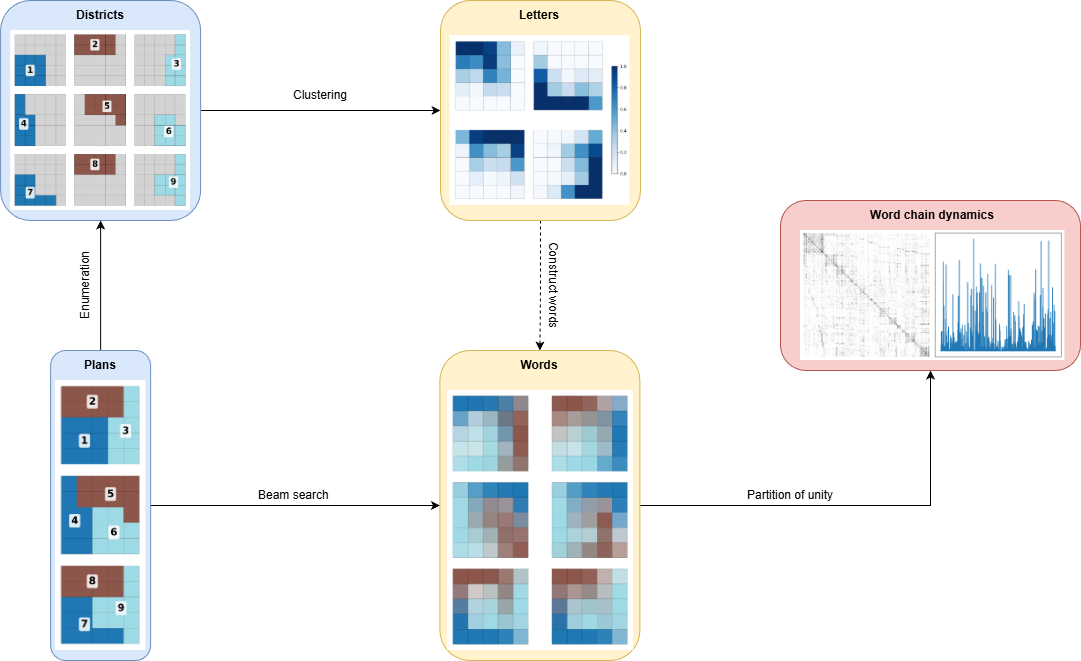
\includegraphics[width=0.92\linewidth]{figures/pipeline_flowchart.png}
    \caption{Overview of the pipeline: districts pooled from an ensemble are clustered into representative district types (letters), each plan is encoded as a unordered tuple of letters (a word), and a beam search enumerates a small neighborhood of candidate words around each plan. A partition of unity over the representative word set then yields stratum weights and a flux matrix summarizing coarse dynamics on words.}
    \label{fig:overlap/pipeline_flowchart}
\end{figure}
\FloatBarrier
